\documentclass[10pt]{amsart}

\usepackage[utf8]{inputenc}

\usepackage[spanish]{babel}
\usepackage{blindtext}

\usepackage{amsmath}
\usepackage{amssymb}
\usepackage{amsfonts}
\usepackage{color}
\usepackage{hyperref}
\usepackage{url}
\usepackage{stmaryrd}
\usepackage{calrsfs}
\usepackage{fancyhdr}
\usepackage{textcomp}
\usepackage{graphicx}
\usepackage{stmaryrd}
\usepackage{lipsum}

\voffset=-1.4mm
\oddsidemargin=14pt
\evensidemargin=14pt
\topmargin=26pt
\headheight=9pt     
\textheight=576pt
\textwidth=441pt %441
\parskip=0pt plus 4pt

\pagestyle{headings}
\title{Proyecto de Programaci\'on Funcional en Haskell}
\author{Programaci\'on Declarativa}
\date{\today}


\begin{document}
	\begin{titlepage}
		\clearpage
		\maketitle
		
		\vspace{3em}
		\begin{center}
			Tema: \textbf{Generador y solucionador de hidatos sudoku} 	

                \vspace{6em}
                \begin{center}
        		
\includegraphics[width=6cm]{haskell.png}
        	\end{center}

			\vspace{6em}
			Autores: \\
			Leandro Rodríguez Llosa \\
			Andry Rosquet Rodríguez
		\end{center}
		\thispagestyle{empty}
	\end{titlepage}

        \normalsize
 
	\small

        \section*{¿Qu\'e es Haskell?}
       
       Haskell es un lenguaje declarativo, orientado a la programaci\'on funcional, los cuales se basan de manera general en el c\'alculo computacional de la funci\'on \href{https://es.wikipedia.org/wiki/C%C3%A1lculo_lambda}{Lamda ($\lambda$)}. Haskell en particular resalta por ser un lenguaje \href{https://es.wikipedia.org/wiki/Programaci%C3%B3n_funcional#Funciones_puras}{funcionalmente puro}, con un tipado \href{https://es.wikipedia.org/wiki/Sistema_de_tipos#:~:text=Se%20dice%20de%20un%20lenguaje,C%2B%2B%2C%20Java%20y%20Haskell.}{est\'atico} \href{https://es.wikipedia.org/wiki/Tipado_fuerte}{fuerte} y una poderosa inferencia de tipos. Entre alguna de las caracter\'isticas m\'as importantes a destacar est\'an la \href{https://es.wikipedia.org/wiki/Transparencia_referencial#:~:text=La%20transparencia%20referencial%20es%20un,diferir%20de%20la%20del%20original%22.}{transparencia referencial},  la t\'ecnica de \href{https://en.wikipedia.org/wiki/Currying}{currying}, el uso de \href{https://wiki.uqbar.org/wiki/articles/orden-superior.html}{funciones de orden superior}, la \href{https://en.wikibooks.org/wiki/Haskell/Pattern_matching}{correspondendia de patrones}, la \href{https://hmn.wiki/es/Lazy_evaluation}{evaluaci\'on perezosa} y las \href{https://cs.famaf.unc.edu.ar/~hoffmann/pd18/practico01.html#tipos-recursivos-y-polim%C3%B3rficos}{funciones y tipos polim\'orficos}. 

        \section*{Hidato sudoku}

        Hidato sudoku, es un juego de lógica inventado por el matemático israelí Dr. Gyora M. Benedek. Un sudoku de este estilo puede adoptar cualquier forma, y est\'a compuesto por un valor m\'inimo (generalmente 1), uno m\'aximo (generalmente la cantidad de celdas), y algunos otros n\'umeros dispersos en el puzzle. El objetivo del juego es llenar las cuadrículas vac\'ias, con números consecutivos que se conectan horizontal, vertical o diagonalmente, y se sabe que existe un \'unico camino que comienza en el valor m\'inimo dado, y termina en el m\'aximo.

        Mir\'andolo desde un enfoque un poco m\'as computacional, se puede ver como un grafo no dirigido y conexo, con algunos nodos vac\'ios y otros con valores, y el problema consiste en encontrar un camino de Hamilton que comienza en el valor m\'inimo que se encuentra en el grafo y termina en el m\'aximo.

        Para entender mejor lo que se estaba explicando anteriormente se deja una imagen donde muestra un hidato no solucionado en el inciso \textit{a)} y su soluci\'on en el \textit{b)}.  

        \begin{center}
            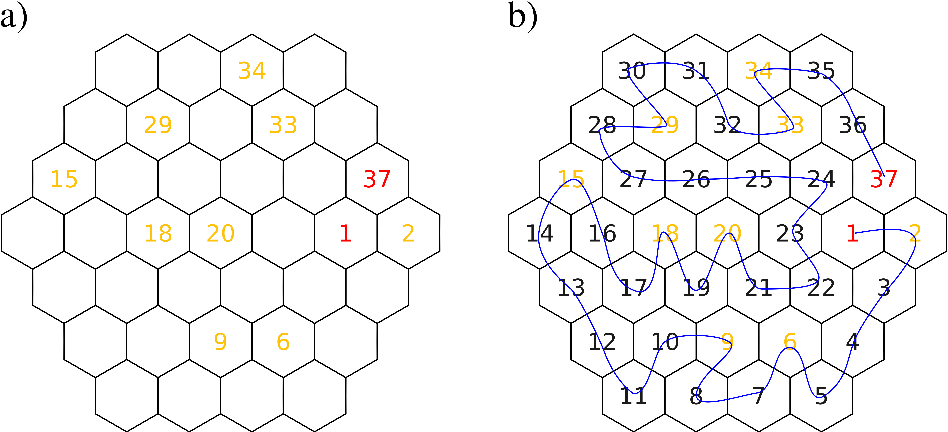
\includegraphics[width=6cm]{hidato-sudoku.png}
        \end{center}

        Para modelar el problema, y representar cualquier figura que se desee, se tienen dos matrices, una con los n\'umeros y otra de m\'ascara marcando en \textit{True} las casilla v\'alidas del juego y en \textit{False} las que no. Para ellos se cre\'o un tipo \textit{Hidato} que modela este concepto.

        \subsection*{Hidato:} este tipo se define para almacenar la informaci\'on referente a un Hidato Sudoku. Entre sus propiedades se tiene una matriz de n\'umeros que representa el tablero (\textit{matrix :: [[Int]]}), una m\'ascara booleana que marca en \textit{False} las casillas que tienen obst\'aculos (\textit{mask :: [[Bool]]}), un entero para tener la cantidad de casillas libres, y otros dos enteros que representan las dimensiones del tablero. 

        El tipo Hidato representa una instancia de la clase de tipos \textit{Show}, y por tanto se redefine la funci\'on \textbf{show} con el objetivo de poder mostrar con facilidad un hidato.
            
	\section*{Generador de hidatos}

        En esta secci\'on abordaremos los aspetos m\'as importantes para generar un hidato v\'alido a partir de un \textit{Template} dado.
	
        \subsection*{Acercamiento general}

        Lo primero que se hace es cargar el \textit{Template} y generar una posici\'on de inicio del sudoku. Esta selecci\'on de una casilla inicial en el tablero se hace de manera aleatoria, haciendo uso del paquete \textit{random} encontrado en m\'odulo \textit{System.Random}. Luego, se comienza en este punto la b\'usqueda de un camino de Hamilton en la matriz. Si la b\'usqueda no fue exitosa, se repite el mismo proceso. 
        
        Una vez se tenga dicho camino de Hamilton se procede a quitar casillas, analizando qué valores son obligatorios en la posici\'on que se encuentran y los que son prescindibles. Al finalizar el proceso anterior tendr\'iamos un tablero con soluci\'on \'unica.
        
        \subsection*{M\'etodos y estrategias}
        El m\'etodo que busca el camino de Hamilton comenzando desde una posici\'on aleatoria es \textit{generateHidato}. Este genera una posici\'on aleatoria con la funci\'on \textit{getRandom}, luego intenta encontrar un camino de Hamilton cualquiera, y si lo halla, genera una soluci\'on \'unica a partir de este, en caso contrario vuelve a intentar generar otro hidato (este proceso recursivo se hace hasta encontrar una soluci\'on v\'alida). 
        
        Luego teniendo el tablero con una soluci\'on v\'alida, se procede a utilizar la funci\'on \textit{findUniqueSolution} la cual utiliza dicho sudoku ([[a]]) y su mask ([[Bool]]) para encontrar un nuevo tablero con espacios vac\'ios que tenga soluci\'on \'unica([[a]]). Dicho m\'etodo busca informaci\'on necesaria y termina llamando a la funci\'on \textit{iteration} la cual l\'ogicamente itera del 2 al m\'aximo posible del tablero, procediendo a realizarle un an\'alisis a cada uno en relaci\'on con su ubicaci\'on en el sudoku resuelto. 
 
        ¿En qu\'e consiste este an\'alisis?
        
        Se procede a remover dicho n\'umero del tablero y se hace un llamado a la funci\'on \textit{solveNumber} que recibe la matriz de n\'umeros actualizada ([[a]]) y su mask ([[Bool]]), devolviendo el n\'umero de soluciones factibles de ese sudoku. Esto conllevar\'ia a dos posibles resultados que son explicados a continuaci\'on y se analizan en la funci\'on \textit{iteration}, la cual se describir\'a a fondo m\'as adelante:
    
        \begin{itemize}
        
            \item Si el resultado es 1 se elimina dicho valor de manera definitiva porque significa que dicho d\'igito siempre, necesariamente, va a ser ubicado en esta posici\'on.
        
            \item Si el resultado es mayor que 1 esto implica que dicho d\'igito debe estar ubicado obligatoriamente en el tablero resultante, de lo contrario si no estuviese fijado generar\'ia m\'ultiples posibles soluciones.
    
        \end{itemize}	
    
        Cuando se realiz\'o dicho an\'alisis a cada valor, se obtendr\'ia el tablero con soluci\'on \'unica donde estar\'an n\'umeros fijados si son necesarios y espacios disponible que solo brindar\'ian soluci\'on v\'alida si se ubican los n\'umeros requeridos.
	 
        Las funciones anteriores se auxilian de otros m\'etodos para funcionar:
	 
    \begin{itemize}

        \item \textit{genRandom:} Esta funci\'on recibe dos valores enteros que corresponden con el l\'imite inferior y superior del intervalo, y devuelve un valor aleatorio comprendido en este. Se utilizan las funciones \textit{randomR} y \textit{getStdRandom} del m\'odulo \textbf{System.Random}, de la siguiente manera:

        \begin{center}
                getRandom x y = getStdRandom \$ randomR (x,y)
        \end{center}

        Cabe destacar que esta funcionalidad fue una de las m\'as desafiantes en el proceso de desarrollo, porque la idea de lo que se quiere hacer rompe con el principio de transparencia referencial. Para lograr cumplir el objetivo planteado, se utilizan los tipos \textit{IO Monad}  que dan acceso a obtener una instancia del tipo \textit{StdGen}, y como esta tiene una variable global que va cambiando su estado en cada llamado a dicha funci\'on, producto a su interacci\'on con un medio externo el cual va variando constantemente, se puede lograr un comportamiento no determinista. Para m\'as informaci\'on sobre lo antes plateando, consulte la \href{https://hackage.haskell.org/package/random-1.2.1.1/docs/System-Random.html#g:5}{documentaci\'on oficial}.  

        \item \textit{searchHamiltonianPath:} Esta funci\'on recibe un hidato, una posici\'on en dicho hidato, una direcci\'on y el tama\~no del camino que se tiene hasta el momento. Esta funci\'on es un algoritmo de Backtrack cl\'asico, que avanza mientras queden casillas libres en el hidato y la nueva posici\'on a la que se mueve es v\'alida. Las direcciones hacia donde se mueven se controlan mediante un tipo definido llamado \textit{Direction}, y las funciones \textit{directionToRow} y \textit{directionToCol} que dada una direcci\'on devuelven el sumando que permite trasladarse en esa direcci\'on. 

        Es importante se\~nalar que este algoritmo es capaz de resolver un tablero de hidato, y para esto, se a\~nade la comprobaci\'on de que antes de trasladarse si alg\'un vecino de la casilla actual es la pr\'oxima casilla del camino que se est\'a formando, entonces se traslada hacia esta posici\'on y se continua el algoritmo. Pero para a\~nadirle mayor robustez a la soluci\'on se decidi\'o crear dos algoritmos distintos, uno para generar el hidato, y otro para solucionarlo.
                        
        \item \textit{Direction:} este es un tipo que se define con el objetivo de modelar un array de direcciones. Junto con ese tipo vienen implementados dos funciones \textit{directionToRow} y \textit{directionToCol}, las cuales retornan dada una direcci\'on el sumando que se necesita sumar a la posici\'on actual para ser desplazado en dicha direcci\'on.

        \newpage
                      
        \item \textit{isValidPosition:} esta funci\'on define un criterio para decidir si una casilla del hidato es v\'alida. Se dice que una casilla es v\'alida si est\'a comprendida en los l\'imites de la matriz, no es un obst\'aculo y la posici\'on es igual a 0 (o sea, no ha sido visitada), o es igual a el tama\~no de paso menos uno, que significa que ser\'a la pr\'oxima casilla por visitar en el camino que se est\'a construyendo. 
                
        \item \textit{replaceHidato:} esta funci\'on recibe un hidato, una posici\'on y un valor, y devuelve otro hidato con este valor insertado en dicha posici\'on. Para la construcci\'on del hidato resultante se hace uso de la funci\'on auxiliar \textit{replaceMatrix}

        \item \textit{replaceMatrix:} esta funci\'on recibe una lista de listas gen\'erica ([[a]]), una posici\'on y un valor gen\'erico tambi\'en. Esta funci\'on hace uso de otra funci\'on auxiliar \textit{replace} la cual reemplaza un valor en una lista ([a]), junto con la estructura \textbf{let - in} primero reemplazando el valor en la fila correspondiente, y luego haciendo uso de la misma funci\'on \textit{replace} se reemplaza ahora la fila completa en la matriz.
        
        \item \textit{iteration:} recibe un entero \textit{x}, el m\'aximo, la posici\'on de \textit{x} en el sudoku resuelto, el tablero y su \textit{mask}. Se encarga de iterar de ese \textit{x} hasta el m\'aximo, analizando que ocurre si se elimina \textit{x} del tablero para finalmente devolver el tablero con soluci\'on \'unica.
        
        \item \textit{solveNumber:} b\'asicamente es el controlador que recibe el tablero, recopila informaci\'on necesaria y luego ejecuta \textit{giveNumber}.
        
        \item \textit{changeState:} recibe un entero, posici\'on de columna y de fila y el tablero actual y devuelve una nueva matriz ([[a]]) con el entero ubicado en la posici\'on recibida.
        
        \item \textit{correctlyPlaced:} recibiendo un valor \textit{x} que ya se encuentra ubicado en el tablero y la posici\'on del antecesor a este brindar\'a \textit{True} si est\'an adyacentes y \textit{False} de lo contrario.
        
        \item \textit{giveNumber:} recibe un entero, el m\'aximo del tablero, posici\'on de la columna y fila del antecesor, una lista de números que ya se encuentran fijados, el tablero y su mask, devolviendo finalmente un entero que representar\'a el n\'umero de soluciones que tiene el tablero actual. Itera por cada n\'umero, solo se detiene si llega al número m\'aximo del tablero, de lo contrario llama a \textit{validPlace} con cada una de las posibles ubicaciones adyacentes al antecesor. Funciona recursivamente sumando el n\'umero de soluciones factibles generadas al ubicar un n\'umero adyacente a su antecesor en las m\'ultiples posibilidades.
	
        \item \textit{validPlace:} recibir\'a un entero \textit{x}, el m\'aximo del tablero, la posici\'on donde se desea ubicar a \textit{x}, la lista de fijados, el tablero y su \textit{mask}. Se encarga de comprobar si la posici\'on dada es v\'alida seg\'un la m\'ascara por medio de \textit{notValidMask} y si la posici\'on no se encuentra ya ocupada en el tablero con \textit{notValidHidato}. Si cumple todos los requisitos entonces se hace un llamado a \textit{giveNumber} con el sucesor y el tablero actualizado con el n\'umero ya ubicado. Lo anterior asegura un ciclo continuo hasta que se haya recorrido cada n\'umero.
	
        \item \textit{notValidMask} y \textit{notValidHidato:} fueron descritas un poco anteriormente pero a mayor profundidad ambas reciben fila y columna, lo cual constituye la posici\'on que se desea comprobar, adem\'as reciben la \textit{mask} y el hidato respectivamente. Proceden a comprobar si la posici\'on es v\'alida, devolviendo \textit{True} si no lo es y \textit{False} de lo contrario.
    
    \end{itemize}
	 
    Algunas funciones de las anteriores utilizan otros m\'etodos para hacer m\'as coherente y sencillo el funcionamiento. Ejemplo: \textit{changeState} utiliza \textit{changeRow} el cual de manera muy descriptiva cambia la fila ubicando un nuevo n\'umero en cierta columna, los m\'etodos \textit{notValidMask} y \textit{notValidHidato} utilizan \textit{checkMask} y \textit{checkHidato} respectivamente para iterar por las filas del tablero y luego una vez encontrada la fila deseada, hacer un llamado de \textit{checkColumn} y \textit{distintZero} respectivamente para encontrar la columna del tablero y as\'i obtener el resultado deseado.
	 
    Adem\'as se utilizan \'utiles como \textit{searchNumber} que localiza un n\'umero dado en el tablero recibido, devolviendo su posici\'on, \textit{searchTop} que dado un tablero devuelve el número m\'aximo que se encuentra ubicado en este, \textit{getRows} y \textit{getColumns} que dada una matriz brinda el n\'umero de filas y columnas respectivamente que esta tiene, \textit{searchUbicated} recibiendo un tablero retorna una lista de enteros que se encuentran ubicados en esta, \textit{biggerThanOne} recibe una fila con enteros y devuelve una lista con los que son mayores que 1 y otros subm\'etodos auxiliares que realizan pequeñas tareas pero contribuyen al funcionamiento del generador.

    \newpage
    
    \section*{Solucionador de tableros}
	 
    \subsection*{Acercamiento general}
	
    Recibiendo un tablero con valores fijados, el 1 y el m\'aximo entre ellos, y la m\'ascara correspondiente a dicho sudoku, el m\'etodo \textit{solve} se encarga de darle soluci\'on. Similar al generador esta funci\'on itera desde 2 al m\'aximo pero en este caso se analiza que ocurre si se ubica el n\'umero en cada posici\'on adyacente a su antecesor, comprobando siempre que sea v\'alida, y luego se avanza a comprobar el sucesor.
	 
    \subsection*{M\'etodos y estrategias}
	
    El iterador solo se detendr\'a cuando se compruebe que el antecesor al m\'aximo se encuentra bien ubicado, una vez haya ocurrido esto significa que tenemos la soluci\'on, de lo contrario se continua comprobando el resto de posiblidades.
	   
    Se utiliza la funci\'on \textit{ubica}, que es la encargada de iterar por todos los n\'umeros y analizar que ocurre si este se fija en cada posici\'on v\'alida adyacente al antecesor por medio de la funci\'on \textit{validPlace}. Si se realiza un an\'alisis cuidadoso es un m\'etodo muy similar a \textit{giveNumber}, con la diferencia que \textit{ubica}, por conveniencia lo que retorna es un booleano y la matriz solucionada, y no un entero con el n\'umero de soluciones. Se utiliza en el resultado ese primer parámetro booleano para en cada llamado recursivo recibir si se encontró solución de ser \textit{True} y \textit{False} en caso contrario.	
   
   \begin{itemize}
        
        \item \textit{ubica:} como se decribi\'o superficialmente, recibir\'a un entero \textit{x}, la posici\'on de su antecesor, el m\'aximo del tablero, la lista de los valores ubicados inicialmente, el sudoku sin resolver y su \textit{mask}. Este de manera recursiva utilizando \textit{validPlace} al igual que \textit{giveNumber}, con la pequeña diferencia que este devuelve la tupla bool-tablero (Bool,[[Int]]), iterar\'a por cada n\'umero hasta el m\'aximo ubicando \textit{x} de manera adyacente a su antecesor y procediendo a comprobar el sucesor. Lo anterior procede ubicando siempre en una posici\'on v\'alida, ya descrita en el generador. 	
    
    \end{itemize}
    
     El solucionador utiliza al igual que el generador funciones como \textit{changeState}, \textit{correctlyPlaced}, \textit{searchTop}, \textit{searchNumber}, \textit{getRows}, \textit{getColumns}, \textit{notValidMask}, \textit{notValidHidato} y muchos otros con exactamente la misma finalidad. 

    \section*{Templates}
    Se define un template como la m\'ascara booleana de un tablero hidato. Este para ser a\~nadido se necesita saber que es v\'alido, y esto se puede comprobar buscando al menos una casilla del tablero desde donde se puede formar un camino de Hamilton, por lo que se utiliza la funci\'on \textit{searchHamiltonianPath:} antes a\~nadida.

    \section*{Ejecuci\'on del software}

    Para encontrar la informacio\'on de apectos m\'as particulares de la ejecuci\'on del software se recomienda dirigirse al directorio ra\'iz del proyecto y apoyerse en la documentaci\'on brindada en el \textit{README.md}.
     
\end{document}